
\def\k{w}
%\def\kluc{kľúč}
\def\put{$\mathop{\mathit{insert}}(\k)$}
\def\find{$\mathop{\mathit{find}}(\k)$}
\def\delete{$\mathop{\mathit{delete}}(\k)$}
\def\trie{trie}
\def\uz{\hbox{\tt\$}}

\section{Písmenkový strom}
\emph{Písmenkový strom} reprezentuje množinu slov. Oproti binárnym 
vyhľadávacím stromom je hlavný rozdiel v tom, že kľúče nie sú uložené 
vo vrcholoch, ale samotná poloha v strome určuje kľúč (slovo). 

% My používame ako abecedu veľké znaky anglickej 
% abecedy a ukončovací znak značíme dolárom (\uz).



\paragraph{Popis.}
Písmenkový strom je \emph{zakorenený strom}, v~ktorom každá hrana obsahuje 
práve jeden znak z abecedy alebo \emph{ukončovací znak}. Teda, každá cesta 
z koreňa do listu so znakmi $w_1, w_2, \ldots, w_n, \uz$ prirodzene 
zodpovedá slovu $w=w_1w_2\cdots w_n$. \emph{Ukončovací znak} je ľubovoľný, 
dopredu dohodnutý symbol, ktorý sa v abecede nenachádza (napr. \uz). 

Písmenkový strom je \emph{asociatívne pole (slovník)}, čiže 
poskytuje tieto tri operácie:
\begin{itemize}
\item \put\ -- pridá do stromu slovo $\k$;
\item \find\ -- zistí, či sa v strome slovo $\k$ nachádza;
\item \delete\ -- odstráni zo stromu slovo $\k$.
\end{itemize}
Všetky operácie začínajú v koreni a ku slovu pridávajú ukončovací znak, 
teda pracujú s reťazcom $\k\uz$. 

Operácia \put\ vloží do stromu vstupný reťazec tak, že z reťazca číta znaky 
a prechádza po príslušných hranách. Ak hrana s daným symbolom neexistuje, 
pridá ju (pozri obr.~\ref{img:trieinsert}).

\begin{figure}
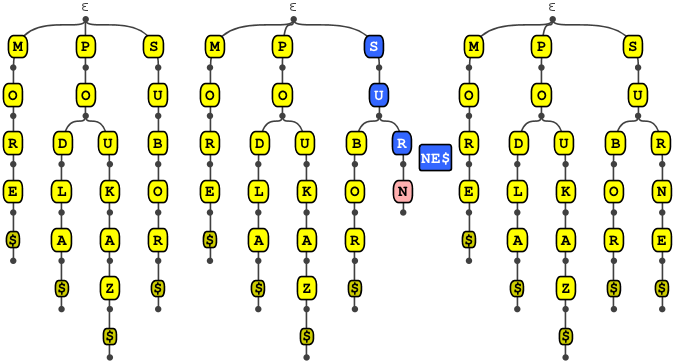
\includegraphics[width=\columnwidth]{obrazky/trieinsertsmall.png}
\caption{\emph{Vloženie slova \uv{{\tt SURNE}}.} Začiatok slova 
\uv{{\tt SU}} sa v strome nachádza, ešte treba pripojiť hrany 
so znakmi {\tt R}, {\tt N}, {\tt E} a \uz.} 
\label{img:trieinsert} 
\end{figure}

Operácia \find\ sa spustí z koreňa podľa postupnosti znakov. Ak hrana, 
po ktorej sa má spustiť neexistuje, dané slovo sa v strome nenachádza. 
Ak prečíta celý vstupný reťazec, dané slovo sa v strome nachádza.

Operácia \delete\ najprv pomocou operácie \find\ zistí umiestnenie slova. 
Ak sa slovo v strome nachádza, algoritmus odstráni hranu s ukončovacím 
znakom a vrchol, ktorý bol na nej zavesený. V tomto štádiu sa nám môže 
stať, že v strome ostane \emph{mŕtva vetva} -- nie je ukončená 
ukončovacím znakom. Pre fungovanie stromu to nevadí, všetky operácie by 
prebiehali správne, ale takto štruktúra zaberá zbytočne veľa miesta. 
Preto je dobré túto mŕtvu vetvu odstrániť (pozri obr.~\ref{img:triedelete}).

\begin{figure}
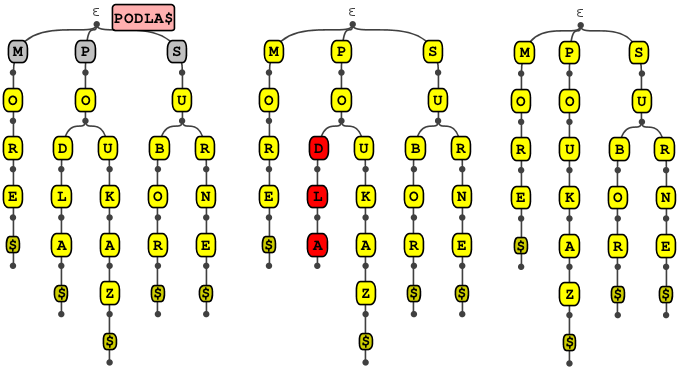
\includegraphics[width=\columnwidth]{obrazky/triedeletesmall.png}
\caption{\emph{Odstránenie slova \uv{{\tt PODLA}}.} Po odstránení 
\uz\ nám v strome ostane nepotrebá prípona \uv{{\tt DLA}} (mŕtva vetva), 
ktorá je vyznačená červenou.}
\label{img:triedelete} 
\end{figure}

\bigskip
% \paragraph{Časová zložitosť.}
Všetky tri operácie majú časovú 
zložitosť $O(|\k|)$, kde $|\k|$ je dĺžka slova.

\paragraph{Použitie.}
Prvýkrát navrhol písmenkový strom \citet{fredkin}, ktorý používal názov 
\emph{trie memory}\footnote{Z anglického re\emph{trie}val -- získanie.}, 
keďže išlo o spôsob udržiavania dát v pamäti. 
%používal operácie 
%$\mathop{storage}$ (\put), $\mathop{retrieval}$ (\find) 
%a $\mathop{deletion}$ (\delete) a dátovú štruktúru nazýval \emph{trie 
%memory}, keďže išlo naozaj o spôsob uloženia dát v pamäti.

%O niečo neskôr \citet{knuth} uviedol vo svojej knihe ako príklad na 
%písmenkový strom vreckový slovník. 
%V tom istom diele uviedol aj možnosť 
%komprimovania vetiev a možnosť prerobenia $m$-árneho \trie\ na binárny. 
%\citet{knuth} však ukázal len komprimovanie koncov vetiev. 
\citet{patricia} navrhol písmenkový strom, v ktorom sa každá cesta bez vetvení
skomprimuje do jedinej hrany (na hranách potom nie sú znaky, ale slová).
Táto štruktúra je známa pod menom \emph{PATRICIA} (tiež \emph{radix tree},
resp.\ \emph{radix trie}) a využíva sa napríklad v \emph{routovacích tabuľkách}
\citep{radix}.

Písmenkový strom (tzv.\ \emph{packed trie} alebo \emph{hash trie}) sa používa
napríklad v programe \TeX\ na slabikovanie slov \citep{liang}.
Pôvodný návrh \citep{fredkin} ako uložiť \trie\ do pamäte zaberal
príliš veľa nevyužitého priestoru. \citet{liang} však navrhol, ako
tieto nároky zmenšiť použitím hašovacej tabuľky.

Písmenkové stromy sa podobajú na \emph{konečné automaty}. 
Vznikli rôzne modifikácie stromov na automaty, ktorých hlavnou výhodou je, 
že v komprimovanej podobe spájajú nielen predpony, ale aj prípony slov 
a teda v slovách ľudských jazykov výrazne znižujú pamäťový priestor potrebný 
na uchovanie dátovej štruktúry. Vďaka tomu sa využívajú na jazykovú korekciu, 
automatické dopĺňanie slov a podobne \citep{scrabble,ca}. 

Priamočiare je použitie písmenkového stromu na utriedenie poľa slov. 
Všetky slová sa pridajú do stromu a potom sa spraví \emph{preorderový prechod} 
stromu. Túto myšlienku spracovali \citet{burstsort1} a veľmi výrazne zrýchlil 
triedenie dlhých zoznamov slov. Neskôr tento algoritmus vylepšili 
\citet{burstsort2}. Kvôli tomu, ako algoritmus pracuje, 
sa nazýva \emph{burstsort}.

% Špeciálnym použitím písmenkového stromu je vytvorenie stromu zo všetkých 
% prípon slova. Táto dátova štruktúra sa nazýva \emph{sufixový strom} a dá sa 
% mo\-di\-fi\-ko\-vať na udržiavanie viacerých slov. Tieto štruktúry majú 
% veľmi veľa praktických využití \citep{gusfield}. 

\paragraph{Vizualizácia.} Pri vizualizácií písmenkového stromu sme použili 
Walkerov algoritumus pre úsporné rozloženie vrcholov v strome. 
\citep{walker} Keď má vrchol viacej synov a hrany kreslíme priamo, tak vzniká 
nedostatok priestoru pre umiestnenie znakov na hrany. Preto sme sa rozhodli 
kresliť hrany zakrivene, podľa Bézierovej krivky určenej štyrmi bodmi. 
Vo vizualizácií sa dajú vložiť náhodné slová podľa momentálne nastaveného 
jazyka. Taktiež sa automaticky odstraňuje diakritika a interpunkcia, takže 
sa dá naraz vložiť súvislý text.
